% Created by tikzDevice version 0.12 on 2019-02-04 12:43:53
% !TEX encoding = UTF-8 Unicode
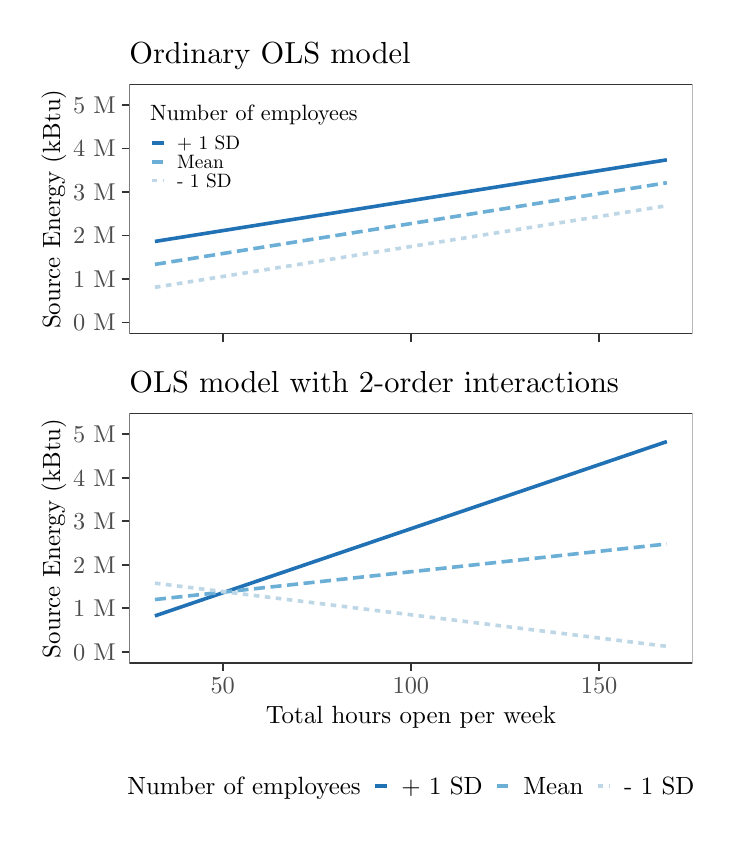
\begin{tikzpicture}[x=1pt,y=1pt]
\definecolor{fillColor}{RGB}{255,255,255}
\path[use as bounding box,fill=fillColor,fill opacity=0.00] (0,0) rectangle (245.72,289.08);
\begin{scope}
\path[clip] (  0.00,170.16) rectangle (245.72,289.08);
\definecolor{drawColor}{RGB}{255,255,255}
\definecolor{fillColor}{RGB}{255,255,255}

\path[draw=drawColor,line width= 0.6pt,line join=round,line cap=round,fill=fillColor] (  0.00,170.16) rectangle (245.72,289.08);
\end{scope}
\begin{scope}
\path[clip] (  0.00,  0.00) rectangle (245.72,170.16);
\definecolor{drawColor}{RGB}{255,255,255}
\definecolor{fillColor}{RGB}{255,255,255}

\path[draw=drawColor,line width= 0.6pt,line join=round,line cap=round,fill=fillColor] (  0.00,  0.00) rectangle (245.72,170.16);
\end{scope}
\begin{scope}
\path[clip] ( 36.74,178.41) rectangle (240.22,268.56);
\definecolor{fillColor}{RGB}{255,255,255}

\path[fill=fillColor] ( 36.74,178.41) rectangle (240.22,268.56);
\definecolor{drawColor}{RGB}{33,113,181}

\path[draw=drawColor,line width= 1.3pt,line join=round] ( 45.99,211.83) --
	( 47.86,212.13) --
	( 49.72,212.43) --
	( 51.59,212.73) --
	( 53.46,213.02) --
	( 55.33,213.32) --
	( 57.20,213.62) --
	( 59.07,213.92) --
	( 60.94,214.22) --
	( 62.80,214.51) --
	( 64.67,214.81) --
	( 66.54,215.11) --
	( 68.41,215.41) --
	( 70.28,215.71) --
	( 72.15,216.00) --
	( 74.02,216.30) --
	( 75.88,216.60) --
	( 77.75,216.90) --
	( 79.62,217.19) --
	( 81.49,217.49) --
	( 83.36,217.79) --
	( 85.23,218.09) --
	( 87.09,218.39) --
	( 88.96,218.68) --
	( 90.83,218.98) --
	( 92.70,219.28) --
	( 94.57,219.58) --
	( 96.44,219.88) --
	( 98.31,220.17) --
	(100.17,220.47) --
	(102.04,220.77) --
	(103.91,221.07) --
	(105.78,221.36) --
	(107.65,221.66) --
	(109.52,221.96) --
	(111.39,222.26) --
	(113.25,222.56) --
	(115.12,222.85) --
	(116.99,223.15) --
	(118.86,223.45) --
	(120.73,223.75) --
	(122.60,224.05) --
	(124.46,224.34) --
	(126.33,224.64) --
	(128.20,224.94) --
	(130.07,225.24) --
	(131.94,225.53) --
	(133.81,225.83) --
	(135.68,226.13) --
	(137.54,226.43) --
	(139.41,226.73) --
	(141.28,227.02) --
	(143.15,227.32) --
	(145.02,227.62) --
	(146.89,227.92) --
	(148.76,228.22) --
	(150.62,228.51) --
	(152.49,228.81) --
	(154.36,229.11) --
	(156.23,229.41) --
	(158.10,229.70) --
	(159.97,230.00) --
	(161.83,230.30) --
	(163.70,230.60) --
	(165.57,230.90) --
	(167.44,231.19) --
	(169.31,231.49) --
	(171.18,231.79) --
	(173.05,232.09) --
	(174.91,232.38) --
	(176.78,232.68) --
	(178.65,232.98) --
	(180.52,233.28) --
	(182.39,233.58) --
	(184.26,233.87) --
	(186.13,234.17) --
	(187.99,234.47) --
	(189.86,234.77) --
	(191.73,235.07) --
	(193.60,235.36) --
	(195.47,235.66) --
	(197.34,235.96) --
	(199.20,236.26) --
	(201.07,236.55) --
	(202.94,236.85) --
	(204.81,237.15) --
	(206.68,237.45) --
	(208.55,237.75) --
	(210.42,238.04) --
	(212.28,238.34) --
	(214.15,238.64) --
	(216.02,238.94) --
	(217.89,239.24) --
	(219.76,239.53) --
	(221.63,239.83) --
	(223.49,240.13) --
	(225.36,240.43) --
	(227.23,240.72) --
	(229.10,241.02) --
	(230.97,241.32);
\definecolor{drawColor}{RGB}{107,174,214}

\path[draw=drawColor,line width= 1.3pt,dash pattern=on 4pt off 2pt on 4pt off 2pt ,line join=round] ( 45.99,203.55) --
	( 47.86,203.84) --
	( 49.72,204.14) --
	( 51.59,204.44) --
	( 53.46,204.74) --
	( 55.33,205.04) --
	( 57.20,205.33) --
	( 59.07,205.63) --
	( 60.94,205.93) --
	( 62.80,206.23) --
	( 64.67,206.53) --
	( 66.54,206.82) --
	( 68.41,207.12) --
	( 70.28,207.42) --
	( 72.15,207.72) --
	( 74.02,208.01) --
	( 75.88,208.31) --
	( 77.75,208.61) --
	( 79.62,208.91) --
	( 81.49,209.21) --
	( 83.36,209.50) --
	( 85.23,209.80) --
	( 87.09,210.10) --
	( 88.96,210.40) --
	( 90.83,210.69) --
	( 92.70,210.99) --
	( 94.57,211.29) --
	( 96.44,211.59) --
	( 98.31,211.89) --
	(100.17,212.18) --
	(102.04,212.48) --
	(103.91,212.78) --
	(105.78,213.08) --
	(107.65,213.38) --
	(109.52,213.67) --
	(111.39,213.97) --
	(113.25,214.27) --
	(115.12,214.57) --
	(116.99,214.86) --
	(118.86,215.16) --
	(120.73,215.46) --
	(122.60,215.76) --
	(124.46,216.06) --
	(126.33,216.35) --
	(128.20,216.65) --
	(130.07,216.95) --
	(131.94,217.25) --
	(133.81,217.55) --
	(135.68,217.84) --
	(137.54,218.14) --
	(139.41,218.44) --
	(141.28,218.74) --
	(143.15,219.03) --
	(145.02,219.33) --
	(146.89,219.63) --
	(148.76,219.93) --
	(150.62,220.23) --
	(152.49,220.52) --
	(154.36,220.82) --
	(156.23,221.12) --
	(158.10,221.42) --
	(159.97,221.72) --
	(161.83,222.01) --
	(163.70,222.31) --
	(165.57,222.61) --
	(167.44,222.91) --
	(169.31,223.20) --
	(171.18,223.50) --
	(173.05,223.80) --
	(174.91,224.10) --
	(176.78,224.40) --
	(178.65,224.69) --
	(180.52,224.99) --
	(182.39,225.29) --
	(184.26,225.59) --
	(186.13,225.89) --
	(187.99,226.18) --
	(189.86,226.48) --
	(191.73,226.78) --
	(193.60,227.08) --
	(195.47,227.37) --
	(197.34,227.67) --
	(199.20,227.97) --
	(201.07,228.27) --
	(202.94,228.57) --
	(204.81,228.86) --
	(206.68,229.16) --
	(208.55,229.46) --
	(210.42,229.76) --
	(212.28,230.06) --
	(214.15,230.35) --
	(216.02,230.65) --
	(217.89,230.95) --
	(219.76,231.25) --
	(221.63,231.54) --
	(223.49,231.84) --
	(225.36,232.14) --
	(227.23,232.44) --
	(229.10,232.74) --
	(230.97,233.03);
\definecolor{drawColor}{RGB}{189,215,231}

\path[draw=drawColor,line width= 1.3pt,dash pattern=on 2pt off 2pt on 2pt off 2pt ,line join=round] ( 45.99,195.26) --
	( 47.86,195.56) --
	( 49.72,195.86) --
	( 51.59,196.15) --
	( 53.46,196.45) --
	( 55.33,196.75) --
	( 57.20,197.05) --
	( 59.07,197.34) --
	( 60.94,197.64) --
	( 62.80,197.94) --
	( 64.67,198.24) --
	( 66.54,198.54) --
	( 68.41,198.83) --
	( 70.28,199.13) --
	( 72.15,199.43) --
	( 74.02,199.73) --
	( 75.88,200.03) --
	( 77.75,200.32) --
	( 79.62,200.62) --
	( 81.49,200.92) --
	( 83.36,201.22) --
	( 85.23,201.51) --
	( 87.09,201.81) --
	( 88.96,202.11) --
	( 90.83,202.41) --
	( 92.70,202.71) --
	( 94.57,203.00) --
	( 96.44,203.30) --
	( 98.31,203.60) --
	(100.17,203.90) --
	(102.04,204.20) --
	(103.91,204.49) --
	(105.78,204.79) --
	(107.65,205.09) --
	(109.52,205.39) --
	(111.39,205.68) --
	(113.25,205.98) --
	(115.12,206.28) --
	(116.99,206.58) --
	(118.86,206.88) --
	(120.73,207.17) --
	(122.60,207.47) --
	(124.46,207.77) --
	(126.33,208.07) --
	(128.20,208.37) --
	(130.07,208.66) --
	(131.94,208.96) --
	(133.81,209.26) --
	(135.68,209.56) --
	(137.54,209.85) --
	(139.41,210.15) --
	(141.28,210.45) --
	(143.15,210.75) --
	(145.02,211.05) --
	(146.89,211.34) --
	(148.76,211.64) --
	(150.62,211.94) --
	(152.49,212.24) --
	(154.36,212.54) --
	(156.23,212.83) --
	(158.10,213.13) --
	(159.97,213.43) --
	(161.83,213.73) --
	(163.70,214.02) --
	(165.57,214.32) --
	(167.44,214.62) --
	(169.31,214.92) --
	(171.18,215.22) --
	(173.05,215.51) --
	(174.91,215.81) --
	(176.78,216.11) --
	(178.65,216.41) --
	(180.52,216.71) --
	(182.39,217.00) --
	(184.26,217.30) --
	(186.13,217.60) --
	(187.99,217.90) --
	(189.86,218.19) --
	(191.73,218.49) --
	(193.60,218.79) --
	(195.47,219.09) --
	(197.34,219.39) --
	(199.20,219.68) --
	(201.07,219.98) --
	(202.94,220.28) --
	(204.81,220.58) --
	(206.68,220.88) --
	(208.55,221.17) --
	(210.42,221.47) --
	(212.28,221.77) --
	(214.15,222.07) --
	(216.02,222.36) --
	(217.89,222.66) --
	(219.76,222.96) --
	(221.63,223.26) --
	(223.49,223.56) --
	(225.36,223.85) --
	(227.23,224.15) --
	(229.10,224.45) --
	(230.97,224.75);
\definecolor{drawColor}{gray}{0.20}

\path[draw=drawColor,line width= 0.6pt,line join=round,line cap=round] ( 36.74,178.41) rectangle (240.22,268.56);
\end{scope}
\begin{scope}
\path[clip] ( 36.74, 59.49) rectangle (240.22,149.64);
\definecolor{fillColor}{RGB}{255,255,255}

\path[fill=fillColor] ( 36.74, 59.49) rectangle (240.22,149.64);
\definecolor{drawColor}{RGB}{33,113,181}

\path[draw=drawColor,line width= 1.3pt,line join=round] ( 45.99, 76.53) --
	( 47.86, 77.16) --
	( 49.72, 77.80) --
	( 51.59, 78.44) --
	( 53.46, 79.07) --
	( 55.33, 79.71) --
	( 57.20, 80.35) --
	( 59.07, 80.98) --
	( 60.94, 81.62) --
	( 62.80, 82.25) --
	( 64.67, 82.89) --
	( 66.54, 83.53) --
	( 68.41, 84.16) --
	( 70.28, 84.80) --
	( 72.15, 85.44) --
	( 74.02, 86.07) --
	( 75.88, 86.71) --
	( 77.75, 87.34) --
	( 79.62, 87.98) --
	( 81.49, 88.62) --
	( 83.36, 89.25) --
	( 85.23, 89.89) --
	( 87.09, 90.53) --
	( 88.96, 91.16) --
	( 90.83, 91.80) --
	( 92.70, 92.43) --
	( 94.57, 93.07) --
	( 96.44, 93.71) --
	( 98.31, 94.34) --
	(100.17, 94.98) --
	(102.04, 95.62) --
	(103.91, 96.25) --
	(105.78, 96.89) --
	(107.65, 97.52) --
	(109.52, 98.16) --
	(111.39, 98.80) --
	(113.25, 99.43) --
	(115.12,100.07) --
	(116.99,100.71) --
	(118.86,101.34) --
	(120.73,101.98) --
	(122.60,102.61) --
	(124.46,103.25) --
	(126.33,103.89) --
	(128.20,104.52) --
	(130.07,105.16) --
	(131.94,105.80) --
	(133.81,106.43) --
	(135.68,107.07) --
	(137.54,107.70) --
	(139.41,108.34) --
	(141.28,108.98) --
	(143.15,109.61) --
	(145.02,110.25) --
	(146.89,110.89) --
	(148.76,111.52) --
	(150.62,112.16) --
	(152.49,112.79) --
	(154.36,113.43) --
	(156.23,114.07) --
	(158.10,114.70) --
	(159.97,115.34) --
	(161.83,115.98) --
	(163.70,116.61) --
	(165.57,117.25) --
	(167.44,117.88) --
	(169.31,118.52) --
	(171.18,119.16) --
	(173.05,119.79) --
	(174.91,120.43) --
	(176.78,121.07) --
	(178.65,121.70) --
	(180.52,122.34) --
	(182.39,122.97) --
	(184.26,123.61) --
	(186.13,124.25) --
	(187.99,124.88) --
	(189.86,125.52) --
	(191.73,126.16) --
	(193.60,126.79) --
	(195.47,127.43) --
	(197.34,128.06) --
	(199.20,128.70) --
	(201.07,129.34) --
	(202.94,129.97) --
	(204.81,130.61) --
	(206.68,131.25) --
	(208.55,131.88) --
	(210.42,132.52) --
	(212.28,133.15) --
	(214.15,133.79) --
	(216.02,134.43) --
	(217.89,135.06) --
	(219.76,135.70) --
	(221.63,136.34) --
	(223.49,136.97) --
	(225.36,137.61) --
	(227.23,138.24) --
	(229.10,138.88) --
	(230.97,139.52);
\definecolor{drawColor}{RGB}{107,174,214}

\path[draw=drawColor,line width= 1.3pt,dash pattern=on 4pt off 2pt on 4pt off 2pt ,line join=round] ( 45.99, 82.44) --
	( 47.86, 82.64) --
	( 49.72, 82.84) --
	( 51.59, 83.04) --
	( 53.46, 83.25) --
	( 55.33, 83.45) --
	( 57.20, 83.65) --
	( 59.07, 83.86) --
	( 60.94, 84.06) --
	( 62.80, 84.26) --
	( 64.67, 84.46) --
	( 66.54, 84.67) --
	( 68.41, 84.87) --
	( 70.28, 85.07) --
	( 72.15, 85.28) --
	( 74.02, 85.48) --
	( 75.88, 85.68) --
	( 77.75, 85.88) --
	( 79.62, 86.09) --
	( 81.49, 86.29) --
	( 83.36, 86.49) --
	( 85.23, 86.70) --
	( 87.09, 86.90) --
	( 88.96, 87.10) --
	( 90.83, 87.30) --
	( 92.70, 87.51) --
	( 94.57, 87.71) --
	( 96.44, 87.91) --
	( 98.31, 88.12) --
	(100.17, 88.32) --
	(102.04, 88.52) --
	(103.91, 88.72) --
	(105.78, 88.93) --
	(107.65, 89.13) --
	(109.52, 89.33) --
	(111.39, 89.54) --
	(113.25, 89.74) --
	(115.12, 89.94) --
	(116.99, 90.14) --
	(118.86, 90.35) --
	(120.73, 90.55) --
	(122.60, 90.75) --
	(124.46, 90.96) --
	(126.33, 91.16) --
	(128.20, 91.36) --
	(130.07, 91.56) --
	(131.94, 91.77) --
	(133.81, 91.97) --
	(135.68, 92.17) --
	(137.54, 92.37) --
	(139.41, 92.58) --
	(141.28, 92.78) --
	(143.15, 92.98) --
	(145.02, 93.19) --
	(146.89, 93.39) --
	(148.76, 93.59) --
	(150.62, 93.79) --
	(152.49, 94.00) --
	(154.36, 94.20) --
	(156.23, 94.40) --
	(158.10, 94.61) --
	(159.97, 94.81) --
	(161.83, 95.01) --
	(163.70, 95.21) --
	(165.57, 95.42) --
	(167.44, 95.62) --
	(169.31, 95.82) --
	(171.18, 96.03) --
	(173.05, 96.23) --
	(174.91, 96.43) --
	(176.78, 96.63) --
	(178.65, 96.84) --
	(180.52, 97.04) --
	(182.39, 97.24) --
	(184.26, 97.45) --
	(186.13, 97.65) --
	(187.99, 97.85) --
	(189.86, 98.05) --
	(191.73, 98.26) --
	(193.60, 98.46) --
	(195.47, 98.66) --
	(197.34, 98.87) --
	(199.20, 99.07) --
	(201.07, 99.27) --
	(202.94, 99.47) --
	(204.81, 99.68) --
	(206.68, 99.88) --
	(208.55,100.08) --
	(210.42,100.29) --
	(212.28,100.49) --
	(214.15,100.69) --
	(216.02,100.89) --
	(217.89,101.10) --
	(219.76,101.30) --
	(221.63,101.50) --
	(223.49,101.71) --
	(225.36,101.91) --
	(227.23,102.11) --
	(229.10,102.31) --
	(230.97,102.52);
\definecolor{drawColor}{RGB}{189,215,231}

\path[draw=drawColor,line width= 1.3pt,dash pattern=on 2pt off 2pt on 2pt off 2pt ,line join=round] ( 45.99, 88.34) --
	( 47.86, 88.11) --
	( 49.72, 87.88) --
	( 51.59, 87.65) --
	( 53.46, 87.42) --
	( 55.33, 87.19) --
	( 57.20, 86.96) --
	( 59.07, 86.73) --
	( 60.94, 86.50) --
	( 62.80, 86.27) --
	( 64.67, 86.04) --
	( 66.54, 85.81) --
	( 68.41, 85.58) --
	( 70.28, 85.35) --
	( 72.15, 85.12) --
	( 74.02, 84.89) --
	( 75.88, 84.65) --
	( 77.75, 84.42) --
	( 79.62, 84.19) --
	( 81.49, 83.96) --
	( 83.36, 83.73) --
	( 85.23, 83.50) --
	( 87.09, 83.27) --
	( 88.96, 83.04) --
	( 90.83, 82.81) --
	( 92.70, 82.58) --
	( 94.57, 82.35) --
	( 96.44, 82.12) --
	( 98.31, 81.89) --
	(100.17, 81.66) --
	(102.04, 81.43) --
	(103.91, 81.20) --
	(105.78, 80.97) --
	(107.65, 80.73) --
	(109.52, 80.50) --
	(111.39, 80.27) --
	(113.25, 80.04) --
	(115.12, 79.81) --
	(116.99, 79.58) --
	(118.86, 79.35) --
	(120.73, 79.12) --
	(122.60, 78.89) --
	(124.46, 78.66) --
	(126.33, 78.43) --
	(128.20, 78.20) --
	(130.07, 77.97) --
	(131.94, 77.74) --
	(133.81, 77.51) --
	(135.68, 77.28) --
	(137.54, 77.05) --
	(139.41, 76.81) --
	(141.28, 76.58) --
	(143.15, 76.35) --
	(145.02, 76.12) --
	(146.89, 75.89) --
	(148.76, 75.66) --
	(150.62, 75.43) --
	(152.49, 75.20) --
	(154.36, 74.97) --
	(156.23, 74.74) --
	(158.10, 74.51) --
	(159.97, 74.28) --
	(161.83, 74.05) --
	(163.70, 73.82) --
	(165.57, 73.59) --
	(167.44, 73.36) --
	(169.31, 73.13) --
	(171.18, 72.89) --
	(173.05, 72.66) --
	(174.91, 72.43) --
	(176.78, 72.20) --
	(178.65, 71.97) --
	(180.52, 71.74) --
	(182.39, 71.51) --
	(184.26, 71.28) --
	(186.13, 71.05) --
	(187.99, 70.82) --
	(189.86, 70.59) --
	(191.73, 70.36) --
	(193.60, 70.13) --
	(195.47, 69.90) --
	(197.34, 69.67) --
	(199.20, 69.44) --
	(201.07, 69.21) --
	(202.94, 68.97) --
	(204.81, 68.74) --
	(206.68, 68.51) --
	(208.55, 68.28) --
	(210.42, 68.05) --
	(212.28, 67.82) --
	(214.15, 67.59) --
	(216.02, 67.36) --
	(217.89, 67.13) --
	(219.76, 66.90) --
	(221.63, 66.67) --
	(223.49, 66.44) --
	(225.36, 66.21) --
	(227.23, 65.98) --
	(229.10, 65.75) --
	(230.97, 65.52);
\definecolor{drawColor}{gray}{0.20}

\path[draw=drawColor,line width= 0.6pt,line join=round,line cap=round] ( 36.74, 59.49) rectangle (240.22,149.64);
\end{scope}
\begin{scope}
\path[clip] (  0.00,  0.00) rectangle (245.72,289.08);
\definecolor{drawColor}{gray}{0.30}

\node[text=drawColor,anchor=base east,inner sep=0pt, outer sep=0pt, scale=  0.88] at ( 31.79,179.48) {0 M};

\node[text=drawColor,anchor=base east,inner sep=0pt, outer sep=0pt, scale=  0.88] at ( 31.79,195.20) {1 M};

\node[text=drawColor,anchor=base east,inner sep=0pt, outer sep=0pt, scale=  0.88] at ( 31.79,210.92) {2 M};

\node[text=drawColor,anchor=base east,inner sep=0pt, outer sep=0pt, scale=  0.88] at ( 31.79,226.64) {3 M};

\node[text=drawColor,anchor=base east,inner sep=0pt, outer sep=0pt, scale=  0.88] at ( 31.79,242.36) {4 M};

\node[text=drawColor,anchor=base east,inner sep=0pt, outer sep=0pt, scale=  0.88] at ( 31.79,258.08) {5 M};
\end{scope}
\begin{scope}
\path[clip] (  0.00,  0.00) rectangle (245.72,289.08);
\definecolor{drawColor}{gray}{0.20}

\path[draw=drawColor,line width= 0.6pt,line join=round] ( 33.99,182.51) --
	( 36.74,182.51);

\path[draw=drawColor,line width= 0.6pt,line join=round] ( 33.99,198.23) --
	( 36.74,198.23);

\path[draw=drawColor,line width= 0.6pt,line join=round] ( 33.99,213.95) --
	( 36.74,213.95);

\path[draw=drawColor,line width= 0.6pt,line join=round] ( 33.99,229.67) --
	( 36.74,229.67);

\path[draw=drawColor,line width= 0.6pt,line join=round] ( 33.99,245.39) --
	( 36.74,245.39);

\path[draw=drawColor,line width= 0.6pt,line join=round] ( 33.99,261.11) --
	( 36.74,261.11);
\end{scope}
\begin{scope}
\path[clip] (  0.00,  0.00) rectangle (245.72,289.08);
\definecolor{drawColor}{gray}{0.30}

\node[text=drawColor,anchor=base east,inner sep=0pt, outer sep=0pt, scale=  0.88] at ( 31.79, 60.56) {0 M};

\node[text=drawColor,anchor=base east,inner sep=0pt, outer sep=0pt, scale=  0.88] at ( 31.79, 76.28) {1 M};

\node[text=drawColor,anchor=base east,inner sep=0pt, outer sep=0pt, scale=  0.88] at ( 31.79, 92.00) {2 M};

\node[text=drawColor,anchor=base east,inner sep=0pt, outer sep=0pt, scale=  0.88] at ( 31.79,107.72) {3 M};

\node[text=drawColor,anchor=base east,inner sep=0pt, outer sep=0pt, scale=  0.88] at ( 31.79,123.44) {4 M};

\node[text=drawColor,anchor=base east,inner sep=0pt, outer sep=0pt, scale=  0.88] at ( 31.79,139.16) {5 M};
\end{scope}
\begin{scope}
\path[clip] (  0.00,  0.00) rectangle (245.72,289.08);
\definecolor{drawColor}{gray}{0.20}

\path[draw=drawColor,line width= 0.6pt,line join=round] ( 33.99, 63.59) --
	( 36.74, 63.59);

\path[draw=drawColor,line width= 0.6pt,line join=round] ( 33.99, 79.31) --
	( 36.74, 79.31);

\path[draw=drawColor,line width= 0.6pt,line join=round] ( 33.99, 95.03) --
	( 36.74, 95.03);

\path[draw=drawColor,line width= 0.6pt,line join=round] ( 33.99,110.75) --
	( 36.74,110.75);

\path[draw=drawColor,line width= 0.6pt,line join=round] ( 33.99,126.47) --
	( 36.74,126.47);

\path[draw=drawColor,line width= 0.6pt,line join=round] ( 33.99,142.19) --
	( 36.74,142.19);
\end{scope}
\begin{scope}
\path[clip] (  0.00,  0.00) rectangle (245.72,289.08);
\definecolor{drawColor}{gray}{0.20}

\path[draw=drawColor,line width= 0.6pt,line join=round] ( 70.47,175.66) --
	( 70.47,178.41);

\path[draw=drawColor,line width= 0.6pt,line join=round] (138.48,175.66) --
	(138.48,178.41);

\path[draw=drawColor,line width= 0.6pt,line join=round] (206.49,175.66) --
	(206.49,178.41);
\end{scope}
\begin{scope}
\path[clip] (  0.00,  0.00) rectangle (245.72,289.08);
\definecolor{drawColor}{gray}{0.20}

\path[draw=drawColor,line width= 0.6pt,line join=round] ( 70.47, 56.74) --
	( 70.47, 59.49);

\path[draw=drawColor,line width= 0.6pt,line join=round] (138.48, 56.74) --
	(138.48, 59.49);

\path[draw=drawColor,line width= 0.6pt,line join=round] (206.49, 56.74) --
	(206.49, 59.49);
\end{scope}
\begin{scope}
\path[clip] (  0.00,  0.00) rectangle (245.72,289.08);
\definecolor{drawColor}{gray}{0.30}

\node[text=drawColor,anchor=base,inner sep=0pt, outer sep=0pt, scale=  0.88] at ( 70.47, 48.48) {50};

\node[text=drawColor,anchor=base,inner sep=0pt, outer sep=0pt, scale=  0.88] at (138.48, 48.48) {100};

\node[text=drawColor,anchor=base,inner sep=0pt, outer sep=0pt, scale=  0.88] at (206.49, 48.48) {150};
\end{scope}
\begin{scope}
\path[clip] (  0.00,  0.00) rectangle (245.72,289.08);
\definecolor{drawColor}{RGB}{0,0,0}

\node[text=drawColor,anchor=base,inner sep=0pt, outer sep=0pt, scale=  0.90] at (138.48, 37.59) {Total hours open per week};
\end{scope}
\begin{scope}
\path[clip] (  0.00,  0.00) rectangle (245.72,289.08);
\definecolor{drawColor}{RGB}{0,0,0}

\node[text=drawColor,rotate= 90.00,anchor=base,inner sep=0pt, outer sep=0pt, scale=  0.90] at ( 11.70,223.48) {Source Energy (kBtu)};
\end{scope}
\begin{scope}
\path[clip] (  0.00,  0.00) rectangle (245.72,289.08);
\definecolor{drawColor}{RGB}{0,0,0}

\node[text=drawColor,rotate= 90.00,anchor=base,inner sep=0pt, outer sep=0pt, scale=  0.90] at ( 11.70,104.56) {Source Energy (kBtu)};
\end{scope}
\begin{scope}
\path[clip] (  0.00,  0.00) rectangle (245.72,289.08);
\definecolor{fillColor}{RGB}{255,255,255}

\path[fill=fillColor] ( 38.77,224.91) rectangle (124.71,267.66);
\end{scope}
\begin{scope}
\path[clip] (  0.00,  0.00) rectangle (245.72,289.08);
\definecolor{drawColor}{RGB}{0,0,0}

\node[text=drawColor,anchor=base west,inner sep=0pt, outer sep=0pt, scale=  0.80] at ( 44.27,255.68) {Number of employees};
\end{scope}
\begin{scope}
\path[clip] (  0.00,  0.00) rectangle (245.72,289.08);
\definecolor{drawColor}{RGB}{33,113,181}

\path[draw=drawColor,line width= 1.3pt,line join=round] ( 44.84,247.32) -- ( 49.40,247.32);
\end{scope}
\begin{scope}
\path[clip] (  0.00,  0.00) rectangle (245.72,289.08);
\definecolor{drawColor}{RGB}{107,174,214}

\path[draw=drawColor,line width= 1.3pt,dash pattern=on 4pt off 2pt on 4pt off 2pt ,line join=round] ( 44.84,240.56) -- ( 49.40,240.56);
\end{scope}
\begin{scope}
\path[clip] (  0.00,  0.00) rectangle (245.72,289.08);
\definecolor{drawColor}{RGB}{189,215,231}

\path[draw=drawColor,line width= 1.3pt,dash pattern=on 2pt off 2pt on 2pt off 2pt ,line join=round] ( 44.84,233.79) -- ( 49.40,233.79);
\end{scope}
\begin{scope}
\path[clip] (  0.00,  0.00) rectangle (245.72,289.08);
\definecolor{drawColor}{RGB}{0,0,0}

\node[text=drawColor,anchor=base west,inner sep=0pt, outer sep=0pt, scale=  0.70] at ( 53.96,244.91) {+ 1 SD};
\end{scope}
\begin{scope}
\path[clip] (  0.00,  0.00) rectangle (245.72,289.08);
\definecolor{drawColor}{RGB}{0,0,0}

\node[text=drawColor,anchor=base west,inner sep=0pt, outer sep=0pt, scale=  0.70] at ( 53.96,238.15) {Mean};
\end{scope}
\begin{scope}
\path[clip] (  0.00,  0.00) rectangle (245.72,289.08);
\definecolor{drawColor}{RGB}{0,0,0}

\node[text=drawColor,anchor=base west,inner sep=0pt, outer sep=0pt, scale=  0.70] at ( 53.96,231.38) {- 1 SD};
\end{scope}
\begin{scope}
\path[clip] (  0.00,  0.00) rectangle (245.72,289.08);
\definecolor{fillColor}{RGB}{255,255,255}

\path[fill=fillColor] ( 30.55,  5.50) rectangle (246.41, 24.64);
\end{scope}
\begin{scope}
\path[clip] (  0.00,  0.00) rectangle (245.72,289.08);
\definecolor{drawColor}{RGB}{0,0,0}

\node[text=drawColor,anchor=base west,inner sep=0pt, outer sep=0pt, scale=  0.90] at ( 36.05, 11.97) {Number of employees};
\end{scope}
\begin{scope}
\path[clip] (  0.00,  0.00) rectangle (245.72,289.08);
\definecolor{drawColor}{RGB}{33,113,181}

\path[draw=drawColor,line width= 1.3pt,line join=round] (125.42, 15.07) -- (129.98, 15.07);
\end{scope}
\begin{scope}
\path[clip] (  0.00,  0.00) rectangle (245.72,289.08);
\definecolor{drawColor}{RGB}{107,174,214}

\path[draw=drawColor,line width= 1.3pt,dash pattern=on 4pt off 2pt on 4pt off 2pt ,line join=round] (169.48, 15.07) -- (174.03, 15.07);
\end{scope}
\begin{scope}
\path[clip] (  0.00,  0.00) rectangle (245.72,289.08);
\definecolor{drawColor}{RGB}{189,215,231}

\path[draw=drawColor,line width= 1.3pt,dash pattern=on 2pt off 2pt on 2pt off 2pt ,line join=round] (205.92, 15.07) -- (210.47, 15.07);
\end{scope}
\begin{scope}
\path[clip] (  0.00,  0.00) rectangle (245.72,289.08);
\definecolor{drawColor}{RGB}{0,0,0}

\node[text=drawColor,anchor=base west,inner sep=0pt, outer sep=0pt, scale=  0.90] at (135.04, 11.97) {+ 1 SD};
\end{scope}
\begin{scope}
\path[clip] (  0.00,  0.00) rectangle (245.72,289.08);
\definecolor{drawColor}{RGB}{0,0,0}

\node[text=drawColor,anchor=base west,inner sep=0pt, outer sep=0pt, scale=  0.90] at (179.10, 11.97) {Mean};
\end{scope}
\begin{scope}
\path[clip] (  0.00,  0.00) rectangle (245.72,289.08);
\definecolor{drawColor}{RGB}{0,0,0}

\node[text=drawColor,anchor=base west,inner sep=0pt, outer sep=0pt, scale=  0.90] at (215.54, 11.97) {- 1 SD};
\end{scope}
\begin{scope}
\path[clip] (  0.00,  0.00) rectangle (245.72,289.08);
\definecolor{drawColor}{RGB}{0,0,0}

\node[text=drawColor,anchor=base west,inner sep=0pt, outer sep=0pt, scale=  1.10] at ( 36.74,276.00) {Ordinary OLS model};
\end{scope}
\begin{scope}
\path[clip] (  0.00,  0.00) rectangle (245.72,289.08);
\definecolor{drawColor}{RGB}{0,0,0}

\node[text=drawColor,anchor=base west,inner sep=0pt, outer sep=0pt, scale=  1.10] at ( 36.74,157.08) {OLS model with 2-order interactions};
\end{scope}
\end{tikzpicture}
